\documentclass[11pt,addpoints,letterpaper]{exam}
\usepackage{adjustbox} % Add this to the preamble
\usepackage{float}

\usepackage{amsmath,tcolorbox,mdframed,xcolor}
\usepackage[top=0.75in, bottom=0.85in, left=1in, right=1in]{geometry} % Adjust margins
\usepackage{mathtools}
\usepackage{siunitx}
\usepackage{nccmath}
\usepackage{physics}
\usepackage{tikz}
\usepackage{multicol}
\usepackage{epigraph}
\usepackage{cancel}
\usepackage{xfrac}
\usepackage{pgfplots}
\usepackage{array}   % For alignment
\usepackage{booktabs} % For better horizontal lines
\usepackage{caption} % For caption formatting
\usepackage{graphicx} % For scaling tables if needed
\usepackage{setspace}

\setlength\epigraphwidth{.8\textwidth}
\setlength\epigraphrule{0pt}

\noprintanswers

\newcommand{\Section}[1]{
\textbf{\\\Large #1\\}
}
\newcommand{\labheader}[4]{%
  \vspace*{-0.2in} % Adjust vertical spacing
  \noindent
  \makebox[0.65\textwidth][l]{Name:\enspace\hrulefill\,\,\,}
  \makebox[0.1\textwidth][l]{\,Period:\enspace}
  \makebox[0.25\textwidth][l]{\hrulefill}\\[0.25cm]
  \makebox[0.65\textwidth][l]{Instructor: \enspace\texttt{\underline{#1}}}\hfill
  \makebox[0.1\textwidth][l]{ Course: }\hfill 
  \makebox[0.25\textwidth][l]{ \texttt{\underline{#2}}}\hfill \\[0.25cm]
  \makebox[0.65\textwidth]{}\makebox[0.1\textwidth][l]{ Term: }\hfill
  \makebox[0.25\textwidth][l]{\enspace\texttt{\underline{#3}}}\hfill
  % \hfill{Score: \underline{\hspace{2cm}}/#4}
  \vspace{0.5in}
}

% Define variables
\newcommand{\instructor}{Mr. Rodriguez}
\newcommand{\coursename}{Conceptual Physics A}
\newcommand{\term}{Winter}
\newcommand{\courseyear}{2024-2025} % Renamed \year to \courseyear to avoid conflict
\newcommand{\instructions}{}
\newcommand{\worksheetname}{Lab 4: Inertia and Oscillations}
\newcommand{\qspppp}{\vspace{6cm}}
\newcommand{\qsppp}{\vspace{4.5cm}}
\newcommand{\qspp}{\vspace{2.5cm}}
\newcommand{\qsp}{\vspace{0.6cm}}

\tcbset{
    myboxstyle/.style={
        colback=white,        % Background color
        colframe=black,       % Border color
        boxrule=0.5pt,        % Border thickness
        arc=5mm,              % Rounding radius
        boxsep=2mm,           % Padding around text
        left=4pt, right=4pt,  % Inner padding on left and right
    }
}
\newcommand{\equationbox}[2]{
\begin{center}
\begin{tcolorbox}[colframe=black!60, colback=white, arc=5mm, boxrule=0.75pt, title=#1]
% \vspace{-0.2in} % Tightens the space between the title and content
\begin{flushleft}
\begin{align}
#2
\end{align}
\end{flushleft}
\end{tcolorbox}
\end{center}
}
\newcommand{\equationboxx}[2]{
\begin{center}
\begin{tcolorbox}[colframe=black!60, colback=white, arc=5mm, boxrule=0.75pt, title=#1]

#2

\end{tcolorbox}
\end{center}
}
\newcommand{\instructionbox}[1]{\begin{center}\fbox{\fbox{{\centering #1}}}\end{center}}

\newcommand{\learningStandard}[1]{
    \small
    \tcbox[colback=gray!10, colframe=black, boxrule=0.5mm, sharp corners=southwest]{
        \textbf{#1} \hspace{0.5cm} % Spacing between title and vertical rule
        \textcolor{gray}{\vrule height 10pt width 0.3pt}\hspace{0.5cm} % Lighter and thinner vertical rule
        \textbf{Score:} \rule{1.5cm}{0.5pt} /10
    }
}

\newtcolorbox{learningStandardBox}[2]{%
    title={Learning Standard #1}, % Title with manual input for the standard number
    fonttitle=\bfseries\small,  % Title font style
    colback=gray!15, % Background color for main content
    colframe=black, % Frame color
    coltitle=black!80, % Font color for title
    colbacktitle=gray!60, % Background color for title
    boxrule=0.5mm, % Border thickness
    sharp corners=south, % Rounded top corners only
    width=\textwidth, % Full text width
    halign=center, % Center-align content
    top=10pt, % Adds extra space at the top to move content down
}
\newcommand{\standardBox}[2]{%
    \begin{learningStandardBox}{#1}{#2} % Passes number and name as arguments
        \begin{minipage}[t]{0.5\textwidth} % Left section for standard name
            \textit{#2} % Italicized name of the standard
        \end{minipage}%
        \hfill
        \begin{minipage}[t]{0.25\textwidth} % Middle section for score
            \textbf{Score:} \rule{1.5cm}{0.5pt} /10
        \end{minipage}%
        \hfill
        \begin{minipage}[t]{0.2\textwidth} % Right section for grade
            \textbf{Grade:} \phantom{1.2cm}
        \end{minipage}
    \end{learningStandardBox}
}
\newcommand{\standardBoxnoscore}[2]{%
    \begin{learningStandardBox}{#1}{#2} % Passes number and name as arguments
        \begin{minipage}[t]{0.5\textwidth} % Left section for standard name
            \textit{#2} % Italicized name of the standard
        \end{minipage}%
        \hfill
        \begin{minipage}[t]{0.25\textwidth} % Middle section for score
            \textbf{Score:} \rule{1.5cm}{0.5pt} /0
        \end{minipage}%
        \hfill
        \begin{minipage}[t]{0.2\textwidth} % Right section for grade
            \textbf{Grade: N/A} \phantom{1.2cm}
        \end{minipage}
    \end{learningStandardBox}
}


\newcommand{\exampleBox}[2]{%
    \begin{tcolorbox}[title=\texttt{Example}]
        \texttt{Problem:} {#1\\} 
        \texttt{Solution:} {#2}
    \end{tcolorbox}%
}

\newcommand{\customsection}[1]{%
    \vspace{1em} % Add some vertical space above (optional)
    {\Large\bfseries #1} % Format the title: large font and bold
    \par\vspace{0.5em}\noindent % Add some space below
}

\addpoints
\printanswers
% BEGIN DOC
\begin{document}

% HEADER
\labheader{Mr. Rodriguez}{Conceptual Physics A}{Winter 2024-25}{\numpoints}

% WORKSHEET NAME
\begin{centering}
\noindent\textbf{\\\Large Midterm Exam Review\\} 
\end{centering}
\qsp
\instructionbox{Be sure to show your work, include units when appropriate, and box your answers.}
\qsp

\standardBox{1}{Scientific Measurement and Estimation}
\qsp
Topics include:
\begin{itemize}
\item The metric system
\item Scientific notation
\item Significant figures
\item Averages
\item Percent Error
\end{itemize}
\qsp

\begin{table}[h!]
\centering

\begin{tabular}{l c c c l}
\toprule
\textbf{Prefix} & \textbf{Symbol} & \textbf{Meaning} & \textbf{Expanded Form} & \textbf{Scientific Form}\\
\midrule
giga- & G & one billion & 1,000,000,000 & $\hspace{4ex}\times 10^{9}$\\ 
mega- & M & one million & 1,000,000 & $\hspace{4ex}\times 10^{6}$\\ 
kilo- & k & one thousand & 1,000 & $\hspace{4ex}\times 10^{3}$\\ 
hecto- & h & one hundred & 100 & $\hspace{4ex}\times 10^{2}$\\ 
-- & -- & one & 1 & $\hspace{4ex}\times 10^{0}$\\ 
centi- & c & one hundredth & 0.01 & $\hspace{4ex}\times 10^{-2}$\\ 
milli- & m & one thousandth & 0.001 & $\hspace{4ex}\times 10^{-3}$\\ 
micro- & $\mu$ & one millionth & 0.000001 & $\hspace{4ex}\times 10^{-6}$\\ 
nano- & n & one billionth & 0.000000001 & $\hspace{4ex}\times 10^{-9}$\\ 
\bottomrule
\end{tabular}
\captionsetup{font=small, labelfont=bf}
\caption{Metric Prefixes Conversion Chart}
\end{table}
\newpage
\Section{LS 1 Sample Questions}
\begin{questions}
\question In your own words, provide at least \textbf{two} reasons as to why the metric system is useful to scientists.  
\ifprintanswers
\begin{solution}
The metric system is the preferred unit system of scientists because
\begin{enumerate}
\item Nearly all countries use it worldwide (save for USA, Myanmar, and Libya) making it a common language for expressing scientific information.
\item All of the base units use the same set of prefixes (\emph{e.g.}, kilo-, centi-).
\item All conversions are connected by factors of ten (\emph{e.g.} $\SI{1}{km}=\SI{e3}{m}$).
\end{enumerate} 
\end{solution} 
\else
\qsppp
\fi


\question
Place either a $<$, $>$, or $=$ sign in the blank.

\begin{parts}
    \part 1 kg \fillin[$>$][1cm] 10 g
    \part 500 g \fillin[$<$][1cm] 1 kg
    \part 2 m \fillin[$=$][1cm] 200 cm
    \part 1 mm \fillin[$<$][1cm] 0.1 m
    \part 1 L \fillin[$=$][1cm] 1000 mL
    \part 1 cm \fillin[$=$][1cm] 10 mm
\end{parts}

\question
Fill in the blank with the correct number.

\begin{parts}
    \part 1 kg = \fillin[$1000$][2cm] g
    \part 5 kg = \fillin[$5000$][2cm] g
    \part 250 g = \fillin[$0.25$][2cm] kg
    \part 1 m = \fillin[$100$][2cm] cm
    \part 1 km = \fillin[$1000$][2cm] m
    \part 15 mm = \fillin[$1.5$][2cm] cm
\end{parts}

\question
Express each of the following in scientific notation:


\begin{parts}
    \part 500 = \fillin[$5.00 \times 10^2$][5cm]
    \part 0.00000012 = \fillin[$1.2 \times 10^{-7}$][5cm]
    \part 7500 = \fillin[$7.5 \times 10^3$][5cm]
    \part 0.02 = \fillin[$2.0 \times 10^{-2}$][5cm]
    \part 123000 = \fillin[$1.23 \times 10^5$][5cm]
\end{parts}

\vspace{0.5cm}

\question
Express each of the following in decimal (expanded) form:

\begin{parts}
    \part $4.56 \times 10^2$ = \fillin[$456$][5cm]
    \part $7.5 \times 10^{-3}$ = \fillin[$0.0075$][5cm]
    \part $3.14 \times 10^5$ = \fillin[$314000$][5cm]
    \part $9.8 \times 10^{-8}$ = \fillin[$0.000000098$][5cm]
    \part $1.2 \times 10^1$ = \fillin[$12$][5cm]
    \part $8.25 \times 10^3$ = \fillin[$8250$][5cm]
\end{parts}

\newpage
\standardBox{2}{Linear Motion}
\qsp

Topics include:
\begin{itemize}
\item Position ($x$), time ($t$), displacement ($\Delta x$), speed ($v = \frac{\Delta x}{\Delta t}$), velocity ($\vb{v}$), and acceleration ($a = \frac{\Delta v}{\Delta t}$). 
\item Interpreting ticker tape data. 
\item Interpreting graphs of motion (position vs. time, speed vs. time). 
\item Converting frequency in Hertz to periods of time in seconds or microseconds. 
\item Free fall due to gravity ($g=\SI{9.8}{m/s^2}$)
\item Kinematics equations:
\qsp
\equationboxx{1D Kinematics Equations}{
\begin{align*}
x(t) &= \frac{1}{2} a t^2 & & \text{(position as a function of time)}\\
v(t) &= at & & \text{(velocity as a function of time)}
\end{align*}
}

\end{itemize}
\qsp 
\Section{LS 2 Sample Questions}
\begin{spacing}{1.5}
\question Speed represents a change in an object's \fillin[position][5cm] divided by its change in \fillin[time][5cm]. \qsp
\question Acceleration represents a change in an object's \fillin[speed][5cm] divided by its change in \fillin[time][5cm]. \qsp
\question The difference between speed and velocity is that speed is a \fillin[scalar][5cm] quantity whereas velocity is a \fillin[vector][5cm] quantity. \qsp
\end{spacing}
\newpage
\question You drop your phone from a height of $\SI{10}{m}$. Take the acceleration of gravity to be $g=\SI{10}{m/s^2}$.
\begin{parts}
\part How long does it take to hit the floor?  
\ifprintanswers
\begin{solution}
Start by identifying the \textbf{knowns} and the \textbf{unknowns}. \qsp 

\textbf{Known:}
\begin{itemize}
\item The height is $x=\SI{10}{m}$.
\item The acceleration is $g=\SI{10}{m/s^2}$.
\end{itemize}
\textbf{Unknown:}
\begin{itemize}
\item The amount of time ($t$) it takes hit the floor. 
\end{itemize}
Now we just need to choose the relevant equation. Looking back to the previous page in the Kinematics Equation box, we see that $x=\frac{1}{2}at^2$ contains the relevant variables. Now we solve for $t$:
\begin{align*}
 \frac{1}{2}gt^2 &= x  & & \text{(position equation)}\\
 g t^2&=2 x  & & \text{(multiply both sides by 2)} \\
 t^2 &=\frac{2 x}{g} & & \text{(divide both sides by $a$)} \\
t &=\sqrt{\frac{2 x}{g}}  & & \text{(take square root of both sides)} \\
t &= \sqrt{\frac{2 \times (\SI{10}{m})}{(\SI{10}{m/s^2})}}  & & \text{(plug in numbers)} \\
t  &\approx \boxed{\SI{1.4}{s}} & & \text{(simplify)} 
\end{align*}
\end{solution} 
\else
\qspp
\fi
\part How fast is it going once it hits the floor? 
\ifprintanswers
\begin{solution}
This time we need the other equation: $v = at$. 

\qsp
\textbf{Known:}
\begin{itemize}
\item The time is $t=\SI{1.4}{s}$.
\item The acceleration is $g=\SI{10}{m/s^2}$.
\end{itemize}
\textbf{Unknown:}
\begin{itemize}
\item The speed $v$ when it hits the floor. 
\end{itemize}
\begin{align*}
v &= at  & & \text{(speed equation)}\\
v &= (\SI{10}{m/s^2})(\SI{1.4}{s})  & & \text{(plug in numbers)} \\
v &= \boxed{\SI{14}{m/s}}  & & \text{(simplify)} 
\end{align*}
\end{solution} 
\else
\qspp
\fi

\ifprintanswers
\begin{solution}

\end{solution} 
\else
\qspp
\fi

\end{parts}

\begin{figure}[H]
    \centering
    % \vspace{0.2cm} % Add vertical space above the image
   \scalebox{1}[1]{ 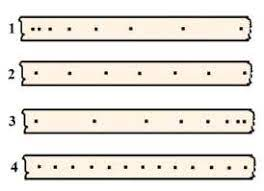
\includegraphics[width=0.45\textwidth]{tickertape.jpeg}} % Specify image width and file name
    % \vspace{0.2cm} % Add vertical space below the image
\end{figure}

\question The above image shows samples from four different ticker tape trials of an object's motion. The starting point of each is on the left-hand side. Fill in the blank below:
\begin{parts}
\part Sample \fillin[1][2cm] represents an object accelerating. \\
\part Sample \fillin[3][2cm] represents an object decelerating. \\
\part Samples \fillin[2][2cm] and \fillin[4][2cm] represent an object moving with constant speed. \\
\begin{spacing}{1.5}
\part Of the samples that represent constant speed, sample \fillin[4][2cm] represents an object moving with a higher speed than sample \fillin[2][2cm].
\end{spacing}
\end{parts}
\newpage
\standardBox{3}{Newton's Laws and Forces}
Topics include:
\begin{itemize}
\item Inertia
\item Newton's Three Laws
\item $\vb{F}=m\vb{a}$
\item Action-reaction pairs
\item Mass ($m$), force ($\vb{F}$), and acceleration ($\vb{a}$). 
\item Net force ($\Sigma F$)
\item Free-body diagrams (force arrow diagrams)
\item Mass ($m$) vs. Weight ($mg$)
\item The normal force ($F_N$)
\item Pulling forces ($F_p$)
\item Static and kinetic coefficients of friction ($\mu_S$ and $\mu_K$)
\item The kinetic friction force ($F_{fr} = \mu_K F_N$)
\end{itemize}
\Section{LS 3 Sample Problems}
\question Inertia is an object's tendency to \fillin[resist a change in motion][10cm]. \qsp
\question State Newton's First Law in your own words. \qsp
\begin{spacing}{1.5}
\question Newton's Second Law says that the net force on an object ($\Sigma F$) is equal to the object's \fillin[mass][5cm] times its \fillin[acceleration][5cm]. \qsp
\end{spacing}
\question You are pushing a crate with a mass of $m=\SI{75}{kg}$. 
\begin{parts}
\part How much force will you need to push with to accelerate the crate at $\SI{0.25}{m/s^2}$? \qspp
\part If you pushed a crate of twice the mass with the same amount of foce, what would its acceleration be? \qspp
\end{parts}
\begin{spacing}{1.5}
\question Newton's Third Law says that every \fillin[action force][5cm] has an equal and opposite \fillin[reaction force][5cm]. \qsp
\end{spacing}
\question Give \textbf{two} examples of action-reaction pairs. \qspp
\question Is your \textbf{mass} the same on Earth as it is on the Moon? What about your \textbf{weight}? Why or why not? \qspp
\question A book is sitting on your desk. It has a mass of $m=\SI{0.5}{kg}$. Take the acceleration of gravity to be $g=\SI{10}{m/s^2}.$
\begin{parts}
\part What is the \textbf{weight} of the book? \qspp
\part What is the \textbf{normal force} ($\vb{F}_N$) that must be provided by the table to keep the book from moving downwards? \qspp
\part Say that the coefficient of static friction between the book and the surface of the table is $\mu_S=0.35$. How much force would you need to push with to get the book to begin to move? \qspp
\part Once the book is moving, you find that you require less force to push it along at a constant speed. Why? \qspp
\end{parts}

\newpage
\standardBox{4}{Momentum}
Topics include:
\begin{itemize}
\item Momentum ($\vb{p} = m\vb{v}$) 
\item The law of conservation of momentum
\item Elastic and inelastic collisions
\item Solving for unknown masses and velocities in collision problems
\end{itemize}
\Section{LS 4 Sample Problems}
\begin{questions}

\question Define momentum in your own words and explain what factors influence it. \qspp

\question Write the equation for momentum ($p$) and define each variable. What are the units of momentum? \qspp

\question State the Law of Conservation of Momentum. \qspp

\question A 1,500 kg car is traveling at 15 m/s. What is its momentum? Show your calculations and include units. \qspp

\question A 2 kg object moving at 3 m/s collides with a stationary 4 kg object. After the collision, the objects stick together. What is their final velocity? (Assume a perfectly inelastic collision and conservation of momentum.) \qspp

\question Describe the difference between elastic and inelastic collisions. Provide a real-world example of each. \qspp

\question A 3 kg ball moving at 6 m/s strikes a 1 kg ball at rest. After the collision, the 3 kg ball moves at 2 m/s. What is the velocity of the 1 kg ball after the collision? (Assume the collision is elastic.) \qspp

\question Two objects of different masses have the same momentum. What can you conclude about their velocities? Explain your reasoning. \qspp



\end{questions}


\end{questions}
\end{document}
